% vim: ft=tex et sts=2 sw=2
%! TEX root = thesis.tex

\chapter{Mathematical Miscellanea}

In this appendix we collect some useful mathematical results and derivations that are frequently referenced to in this dissertation.
For more detailed discussions, refer to standard references in the theory of manifolds, measure theory, and semiclassical physics.

\section{Manifolds}

A manifold, roughly speaking, a set that looks Euclidean\footnote{It is often said that manifolds are smooth sets that look locally ``flat'' and hence can be mapped to an open set in Euclidean space.
This is a bit misleading as the case of the sphere $S^2$ illustrates.
The entire northern hemisphere (except the north pole) of $S^2$ can be mapped to the real plane $\mathbb{R}^{2}$ using stereographic projection.
This means that the two hemispheres of $S^2$ can be covered entirely using two charts.
But neither hemispheres are flat structures.
Flatness also reminds me of curvature, which isn't required for the definition of a smooth manifold, which is much more primitive structure.}

A \emph{regular point} is a point in the domain $X$ where the Jacobian of the map is full rank.
A \emph{regular value} is a point $y \in Y$ such that the Jacobian of all the points in the preimage $f^{-1}(y) \subset X$ is full rank.
Sard's theorem ensures that almost all points in $Y$ are regular values.
%
\begin{theorem}[Sard's theorem]
  The set of critical values of any smooth map $f: X \to Y$, has zero measure in the codomain $Y$.
\end{theorem}

In other words, almost all points in $Y$ are regular values.
As an example, consider $f: \mathbb{R} \to \mathbb{R}$ defined by $x \mapsto x^3 - x$.
The Jacobian in this case is simply the derivative $f'(x) = 3x^2 - 1$, which vanishes only for $x = 3^{-1/2}$.
Hence, every point other than $x = 3^{-1/2}$ is a regular point.%
\footnote{A word of warning is appropriate here: Sard's theorem does not imply that the set of critical points in the domain $X$ is a measure zero subset.
For example, if we consider a constant map, say $f(x) = c \in Y$, then all points in $X$ are critical points.}

One might be tempted to apply the regular value theorem to the energy function itself.
But this wouldn't work since for $E=\|\bm{f}\|^2$ to vanish, $\bm{f}$ must itself vanish, which in turn would make $\nabla E = 2 \bm{f}\nabla\bm{f} = \bm{0}$, making it impossible to apply the regular value theorem on the energy function.

The dimension of tangent space is commonly called a \ac{dof}.

\begin{theorem}[Preimage theorem]
\end{theorem}

\section{Laplace's method}

To evaluate
%
\begin{equation}
  \int_{a}^{b} \dd{x}\, g(x) e^{-\beta U(x)},
\end{equation}
when $\beta$ is large, we first expand $U(x)$ to $\mathcal{O}(x^{2})$ around a critical point $x_{0}$ with $U'(x_{0}) = 0$.
This turns the above integral into a standard Gaussian integral
%
\begin{equation}
  \int_{a}^{b} \dd{x}\, g(x_{0}) \exp\left\{-\beta\left[U(x_{0}) +  U''(x_{0})(x-x_{0})^{2}\right]\right\},
\end{equation}

\begin{figure}
  % \begin{center}
  %   \includegraphics[scale=1.0]{file}
  % \end{center}
  \caption{Plot of the function $U(x) = 9x^{2} + \sin^{2}{3x} + (1-x)\sin^{2}{6x}$ and $e^{-\beta U(x)}$ in the interval $[-1,1]$ for $\beta = 0.1, 0.2, \ldots, 6.4$.  For larger values of $\beta$ the plot is clearly indistinguishable from that of a Gaussian with a width of $U''(0)$.}
  \label{fig:}
\end{figure}

\subsection{Degenerate case}

\section{Coarea formula}

Jacobian determinants are the corrective factors relating the elements of areas of the domains and images of functions (Morgan's book).

The coarea formula,\footnote{Sometimes the coarea formula is misleadingly written~\cite{hartmann2007,hartmann2007a} with the determinant of $(\nabla\hat{\xi})\trans\nabla\hat{\xi}$ in the denominator.  But the Jacobian $\nabla\hat{\xi}$ does not have full column rank when $m < n$ and the determinant $\det\,(\nabla\hat{\xi})\trans\nabla\hat{\xi}$ vanishes.}
%
\begin{theorem}[Coarea formula]
  Given an integrable function $\phi: \mathbb{R}^n \to \mathbb{R}$ and
  Consider a map $\hat{\xi}: \mathbb{R}^n \to \mathbb{R}^m$ (with $m \leq n$) whose level sets foliate $N \subseteq \mathbb{R}^{n}$ we have
  \begin{equation}
    \begin{aligned}
      \int_{\mathbb{R}^n} \dd{\bm{q}}\, \phi(\bm{q}) &= \int_{\mathbb{R}^m} \dd{\xi}\,\int_{\mathbb{R}^n} \dd{\bm{q}}\, \delta\left[\hat{\xi}(\bm{q}) - \xi\right] \phi(\bm{q})\\
                                                     &= \int_{\mathbb{R}^m} \dd{\xi}\,\int_{\bm{q} \in \hat{\xi}^{-1}(\xi)} \frac{\dd{\Omega(\bm{q})}}{|\det \nabla\hat{\xi}(\nabla\hat{\xi})^\mathsf{T}|^{1/2}} \phi(\bm{q})\,,
    \end{aligned}
  \end{equation}
  where $\dd\Omega(\bm{q})$ is the area element on the level set $\hat{\xi}^{-1}(\xi)$.
\end{theorem}
\begin{proof}
  %
  \begin{equation}
    \begin{aligned}
      \int_{\mathbb{R}^{n}} \dd\bm{q}\,\delta\left[\hat{\xi}(\bm{q}) - \xi\right] \phi(\bm{q}) &=
      \lim_{\alpha \to \infty} \left(\frac{\alpha}{2\pi}\right)^{m} \int_{\mathbb{R}^{n}} \dd\bm{q}\, \exp\left(-\tfrac{1}{2}\alpha\Abs{\hat{\xi}(\bm{q}) - \xi}^{2}\right) \phi(\bm{q})
    \end{aligned}
  \end{equation}
  %
  \qed
\end{proof}

Foliation intuitively means that there is a unique hypersurface that passes through each point.

\begin{example}[Integration in polar coordinates]
  As a simple illustration of the coarea formula, consider evaluating the double integral $\int_{\mathbb{R}^{2}} \dd{x}\dd{y}\, \phi(x,y)$, where $\phi(x, y)$ is some integrable function of $(x, y)$.
  The standard polar angle $\theta$ can be computed using the map $\hat{\theta}(x, y) = \tan^{-1}(x, y)$.\footnote{Here $\tan^{-1}(x, y): \mathbb{R}^{2} \setminus \{(0,0)\} \to (-\pi, \pi]$ is the two-argument variant of the inverse tangent, sometimes denoted as $\mathrm{atan2}(y, x)$ in numerical software.  We cannot use $\tan^{-1}(y/x)$ to compute $\theta$ since the range of principal values of $\tan^{-1}(\cdot)$ is conventionally restricted to $(-\pi/2, \pi/2)$.}
  The level set $\hat{\theta}^{-1}(\theta)$ is a straight line starting at the origin (but excluding it) and making an angle of $\theta$ with the positive $x$ axis.
  It is clear that for values of $\theta \in (-\pi, \pi]$, these level sets foliate the entire $\mathbb{R}^{2}$ plane (excluding the origin).
  Choose $\xi = \theta$ and $\hat{\xi}(x, y) = \hat{\theta}(x, y)$ so that
  %
  \begin{equation}
    \int_{\mathbb{R}^{2}} \dd{x}\dd{y}\, \phi(x, y) = \int_{-\pi}^{\pi} \dd\theta\, \int_{\mathbb{R}^{2}} \dd{x}\dd{y}\, \delta[\tan^{-1}(x, y) - \theta] \phi(x, y).
  \end{equation}
  %
  Now, $\nabla\hat{\theta} = \nabla\tan^{-1}(x, y) = (x^{2} + y^{2})^{-1}\begin{pmatrix}-y & x\end{pmatrix}$.
  We can parameterize the points on $\hat{\theta}^{-1}(\theta)$ in terms of $r > 0$ as $(r\cos{\theta}, r\sin{\theta})$.
  Then, $\nabla\hat{\theta} = r^{-1}\begin{pmatrix}-\sin\theta & \cos\theta\end{pmatrix}$ and $\det\,\nabla\hat{\theta}(\nabla\hat{\theta})\trans = r^{-2}$.
  Putting this in the coarea formula and noting that the surface measure on $\hat{\theta}^{-1}(\theta)$ is just $\dd{r}$, we arrive at
  \begin{equation}
    \int_{\mathbb{R}^{2}} \dd{x}\dd{y}\, \phi(x, y) = \int_{-\pi}^{\pi} \dd\theta\, \int_0^{\infty} \dd{r}\, r \phi(r, \theta),
  \end{equation}
  which is the standard double integral of a function expressed in polar coordinates.\footnote{A similar example is discussed in many books on field theory in the context of the Fadeev--Popov method, e.g., the ones by \citet[Section 7.2]{ryder1996} and \citet[Part III.4]{zee2010}.}
  \altqed
\end{example}

Other examples: density of states.  See paper~\cite{gillespie1983}.


\begin{figure}
  \begin{center}
    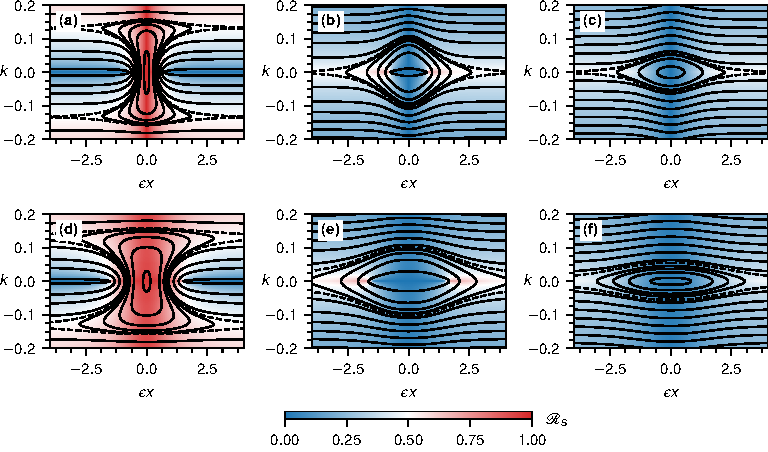
\includegraphics{shell_rays.pdf}
  \end{center}
\end{figure}

For e.g. hello world

\
\section{Operators and symbols}

An operator-symbol correspondence is an association between operators defined on some Hilbert space and ordinary $c$-numbered functions on the phase space, called symbols~\cite[\S 2.3.1]{chaichian2001}.

The symmetrized product $\big\llbracket \hat{\mathsf{A}}_{1}^{k_{1}} \hat{\mathsf{A}}_{2}^{k_{2}} \cdots \hat{\mathsf{A}}_{n}^{k_n} \big\rrbracket$ of $n$ noncommuting operators $\hat{\mathsf{A}}_{i}$ is defined as the coefficient of
%
\begin{equation}
  \frac{k!}{k_{1}!k_{2}!\cdots k_{n}!} a_{1}^{k_{1}} a_{2}^{k_{2}} \cdots a_{n}^{k_{n}}
\end{equation}
%
in the multinomial expansion of $\left(a_{1}\hat{\mathsf{A}}_{1} + a_{2}\hat{\mathsf{A}}_{2} + \cdots + a_{n}\hat{\mathsf{A}}_{n}\right)^{k}$ with $k = k_{1} + k_{2} + \cdots + k_{n}$.

\subsection{Weyl symbols}

\begin{example}
  For a one-dimensional operator $\hat{\mathsf{A}} = a\hat{x}^{n}$, with $a \in \mathbb{C}$ and $n \in \mathbb{Z}$, on making use of $\bra{x + \frac{1}{2}s}a\hat{x}^{n}\ket{x - \frac{1}{2}s} = a \left(x - \frac{1}{2}s\right)^{n}\braket{x + \frac{1}{2}s | x - \frac{1}{2}s} = a\left(x - \frac{1}{2}s\right)^{n} \delta(s)$ in Eq.~XXX, we find $\mathsf{A} = a x^{n}$.
  This also means that the operator $\hat{\mathsf{A}} = \sum_{n} a_{n}\hat{x}^{n}$, which is a polynomial in $\hat{x}$, with $a_{n}$ being the coefficients, has the symbol
  $\mathsf{A} = \sum_{n} a_{n}{x}^{n}$, an ordinary polynomial in $x$.
  More generally, in $d$ dimensions, if $\hat{\mathsf{A}}$ is a multivariate polynomial in the components of $\hat{\bm{x}}$, i.e., $\hat{\mathsf{A}} = \sum_{n_{i}} a_{n_{1}n_{2}\cdots n_{d}} \hat{x}_{1}^{n_{1}}\hat{x}_{2}^{n_{2}}\cdots \hat{x}_{d}^{n_{d}}$, then the corresponding Weyl symbol is $\mathsf{A} = \sum_{n_{i}} a_{n_{1}n_{2}\cdots n_{d}} {x}_{1}^{n_{1}}{x}_{2}^{n_{2}}\cdots {x}_{d}^{n_{d}}$.%
  \footnote{Here, we could have alternatively considered the operator $\sum_{n} a_{n} \hat{\bm{x}}^{n}$, but raising a vector operator to a power is not readily obvious.
    In any case, the generalization we have considered does cover common cases such as $\hat{\mathsf{A}} = \hat{\bm{x}}\cdot\hat{\bm{x}}$.
  In this case, in two dimensions, for instance, the polynomial coefficients will all be zero except for $a_{20} = 1$ and $a_{02} = 1$, and the Weyl symbol would trivially be $x_{1}^{2} + x_{2}^{2}$.}
\end{example}

\section{Star product of symbols}

How can we express the symbol of the product of two operators in terms of their individual symbols?
For example, if $\hat{\mathsf{C}} = \hat{\mathsf{A}}\hat{\mathsf{B}}$, then how is $\mathsf{C}$ related to $\mathsf{A}$ and $\mathsf{B}$?
There is no apriori reason to assume that $\mathsf{C} = \mathsf{A}\mathsf{B}$, and indeed $\mathsf{C} \neq \mathsf{A}\mathsf{B}$, in general.
%
\begin{equation}
  \mathsf{C}(x, k) = 2\int \dd{x'}\, \dd{x''} \,e^{-2ikx} \bra{x + x'}\hat{\mathsf{A}}\ket{x''}\bra{x''}\hat{\mathsf{B}}\ket{x - x'}.
\end{equation}
%
Above we have set $x' \to 2x'$ in the usual Wigner transform expression.
Using the Weyl transform to express the matrix elements $\bra{x + \frac{1}{2}x'}\hat{\mathsf{A}}\ket{x''}$ and $\bra{x''}\hat{\mathsf{B}}\ket{x - \frac{1}{2}x'}$ in terms of the symbols $\mathsf{A}$ and $\mathsf{B}$, we find
%
\begin{equation}
  \begin{aligned}
    \mathsf{C}(x, k) = \frac{2}{(2\pi)^{2}}& \bigg\{\int \dd{x'}\, \dd{x''}\, \dd{k_{1}}\, \dd{k_{2}}\,e^{-2i[kx - k_{1}(x + x' - x'') - k_{2}(-x + x' + x'')]}\\
                                           &\qquad\times \mathsf{A}\left[\tfrac{1}{2}(x + x' + x''), k_{1}\right]\, \mathsf{B}\left[\tfrac{1}{2}(x - x' + x''), k_{2}\right]\bigg\}.
  \end{aligned}
\end{equation}
%
Setting $x_{1} = \frac{1}{2}(x + x' + x'')$ and $x_{2} = \frac{1}{2}(x - x' + x'')$ and changing variables, we find\footnote{An extra Jacobian factor equal to 2 appears while transforming $(x', x'') \to (x_{1}, x_{2})$~\cite[Eq.~(2.3.23) and Problem~2.3.8]{chaichian2001}}
%
\begin{equation}
  \begin{aligned}
    \mathsf{C}(x, k) &= \frac{1}{\pi^{2}} \int \dd{x_{1}}\, \dd{x_{2}}\, \dd{k_{1}}\, \dd{k_{2}}\,e^{-2i[(k_{1} - k)(x_{2} - x) - (k_{2} - k)(x_{1} - x)]} \mathsf{A}(x_{1}, k_{1})\, \mathsf{B}(x_{2}, k_{2})\\
                     &= \frac{1}{\pi^{2}} \int \dd{x_{1}}\, \dd{x_{2}}\, \dd{k_{1}}\, \dd{k_{2}}\,e^{2i(k_{2}x_{1} - k_{1}x_{2})}\,e^{2i(kx_{2} - k_{2}x)} \mathsf{A}(x_{1}, k_{1})\, \mathsf{B}(x + x_{2}, k + k_{2}).\label{eq:moyal1}
  \end{aligned}
\end{equation}
%
In the last step, we have set $x_{2} \to x + x_{2}$ and $k_{2} \to k + k_{2}$, with the hope of Taylor expanding $\mathsf{B}$ around $(x, k)$.
Note that
%
\begin{equation}
  \begin{aligned}
    \mathsf{B}(x + x_{2}, k + k_{2}) &= \mathsf{B}(x, k) + [\partial_{x} \mathsf{B}(x, k)]x_{2} + [\partial_{k} \mathsf{B}(x, k)] k_{2} + \tfrac{1}{2} [\partial^{2}_{x} \mathsf{B}(x, k)] x_{2}^{2}\\
    &\qquad + \tfrac{1}{2} [\partial^{2}_{k} \mathsf{B}(x, k)] k_{2}^{2} + [\partial_{x}\partial_{k} \mathsf{B}(x, k)] x_{2}k_{2} + \cdots \\
    &= \left[1 + x_{2}\partial_{x} + \tfrac{1}{2}x_{2}^{2}\partial^{2}_{x} + \cdots \right]\,
  \left[1 + k_{2}\partial_{k} + \tfrac{1}{2}k_{2}^{2}\partial^{2}_{k} + \cdots \right] \mathsf{B}(x, k)\\
    &= e^{x_{2}\partial_{x}} e^{k_{2}\partial_{k}} \mathsf{B}(x, k).\label{eq:moyal2}
  \end{aligned}
\end{equation}
%
Above, we have made use of the fact that the partial derivatives are with respect to $x$ and $k$ so that $x_{2}$ and $k_{2}$ can be treated as constants that can be moved around.
To simplify this further, we introdue new notation: the operators $\ogets{\partial_{x}}$ and $\ogets{\partial_{k}}$ act \emph{only} on the terms to their left and operators $\oto{\partial_{x}}$ and $\oto{\partial_{k}}$ act \emph{only} on the terms to their right.
Then,
%
\begin{equation}
  \begin{aligned}
    e^{-2ik_{2}x} e^{\frac{i}{2}\ogets{\partial_{x}}\oto{\partial_{k}}} &= e^{-2ik_{2}x} \left[1 +  \tfrac{i}{2}\ogets{\partial_{x}}\oto{\partial_{k}} - \tfrac{1}{8}\ogets{\partial^{2}_{x}}\oto{\partial^{2}_{k}} + \cdots \right]\\
                                                            &= e^{-2ik_{2}x} \left[1 +  k_{2}\oto{\partial_{k}} + \tfrac{1}{2}k_{2}^{2}\oto{\partial^{2}_{k}} + \cdots \right]\\
                                                            &= e^{-2ik_{2}x}e^{k_{2}\partial_{k}}
  \end{aligned}\label{eq:moyal3}
\end{equation}
%
Similarly, we see that
%
\begin{equation}
  e^{2ikx_{2}}e^{-\frac{i}{2}\ogets{\partial_{k}}\oto{\partial_{x}}} = e^{2ikx_{2}}e^{x_{2}\partial_{x}}.\label{eq:moyal4}
\end{equation}
%
Using Eqs.~\eqref{eq:moyal2}--\eqref{eq:moyal4}, and defining $\hat{\mathcal{L}} = \ogets{\partial_{x}} \oto{\partial_{k}} - \ogets{\partial_{k}}\oto{\partial_{x}}$, we can turn Eq.~\eqref{eq:moyal1} into
%
\begin{equation}
  \begin{aligned}
    \mathsf{C}(x, k) &= \frac{1}{\pi^{2}} \left[\int \dd{x_{1}}\, \dd{k_{1}}\, \dd{x_{2}}\, \dd{k_{2}}\,e^{2i[k_{2}(x_{1} - x) - x_{2}(k_{1} - k)]} \mathsf{A}(x_{1}, k_{1})\, e^{\frac{i}{2}\hat{\mathcal{L}}}\right] \mathsf{B}(x, k)\\
                     &= \left[\int \dd{x_{1}}\, \dd{k_{1}}\, \delta(x_{1} - x)\,\delta(k_{1} - k) \mathsf{A}(x_{1}, k_{1})\, e^{\frac{i}{2}\hat{\mathcal{L}}}\right] \mathsf{B}(x, k)\\
                     &= \mathsf{A}(x, k)e^{\frac{i}{2}\hat{\mathcal{L}}} \mathsf{B}(x, k).
  \end{aligned}
\end{equation}
%
In the first step above, we have put brackets around the integral (which is now an operator) to emphasize that $\mathsf{B}(x, k)$ can be taken outside it.
The final step defines the Moyal (or ``star'' $\star$) product, which can be used to compute the symbol of the product of two operators in terms of their respective symbols:
%
\begin{equation}
  \begin{aligned}
    \mathsf{C}(x, k) = \mathsf{A}(x, k)\star\mathsf{B}(x, k) &= \mathsf{A}(x, k)e^{\frac{i\epsilon}{2}\hat{\mathcal{L}}} \mathsf{B}(x, k)\\
                                                             &= \mathsf{A}(x, k)\left[1 + \frac{i\epsilon}{2}\left(\ogets{\partial_{x}}\oto{\partial_{k}} - \ogets{\partial_{k}}\oto{\partial_{x}}\right) + \mathcal{O}(\epsilon^{2}) \right] \mathsf{B}(x, k)\\
                                                             &= \mathsf{A}(x, k)\mathsf{B}(x, k) + \frac{i\epsilon}{2}\left\{\mathsf{A}(x, k), \mathsf{B}(x, k)\right\} + \mathcal{O}(\epsilon^{2}).
  \end{aligned}
\end{equation}
